\section{进阶教程(本节部分内容供有编程经验的用户参考)}
\label{section_advanced_usage}

\subsection{关于控制器}\footnote{此部分内容有待进一步完善。}

控制器接收以下命令行参数(视版本而定)。请在 \lstinline{Controller.ps1} 中向 \lstinline{Controller.exe} 传入命令行参数(下面的例子遵循 Powershell 语法):

\begin{itemize}
\item \lstinline{--GameRootDirectory} 游戏安装根目录,如不指定则会自动检测(如非必要,不应使用此参数)。路径需要使用引号包含,如:\lstinline{"C:\csol"}。
\item \lstinline{--LaunchGameCmd} 启动游戏的命令,如不指定则会自动检测(如非必要,不应使用此参数)。启动命令需要使用引号包含,当需要为启动器指定命令行选项时,启动器路径本身还需要额外使用引号以分隔启动器路径和启动器接收的命令行参数。如:\lstinline{"`"C:\TCGame\TCGame.exe`" cso"}。
\item \lstinline{--MaxWaitTimeInRoom} 在房间内等待的最长时间,单位为秒,如不指定则默认为 900。当房主长时间未开始游戏(房间超过 15 分钟未开始游戏会自动关闭),达到此参数设定的超时时间时,将离开当前房间自行创建新的房间挂机。
\end{itemize}

例如,图 \ref{ch7fig-change-max-wait-time-in-room-0} 中将在房间内等待的最长时间设置为 300 秒。重新运行 \lstinline{Controller.ps1} 即可生效(图 \ref{ch7fig-change-max-wait-time-in-room-1})。

\begin{figure}[H]
    \Centering
    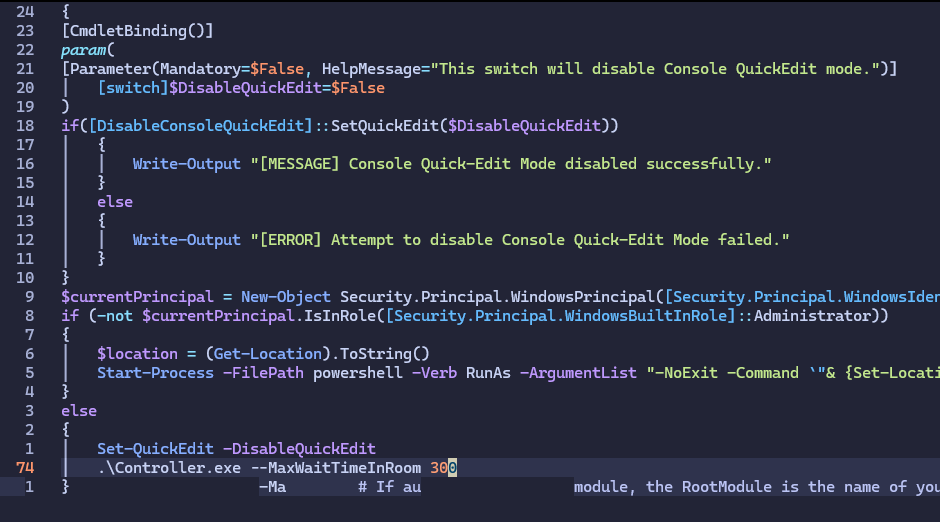
\includegraphics[width=\textwidth]{docs/assets/advanced/change_max_wait_time_in_room_0.png}
    \caption{修改在房间内等待的最长时间}
    \label{ch7fig-change-max-wait-time-in-room-0}
\end{figure}

\begin{figure}[H]
    \Centering
    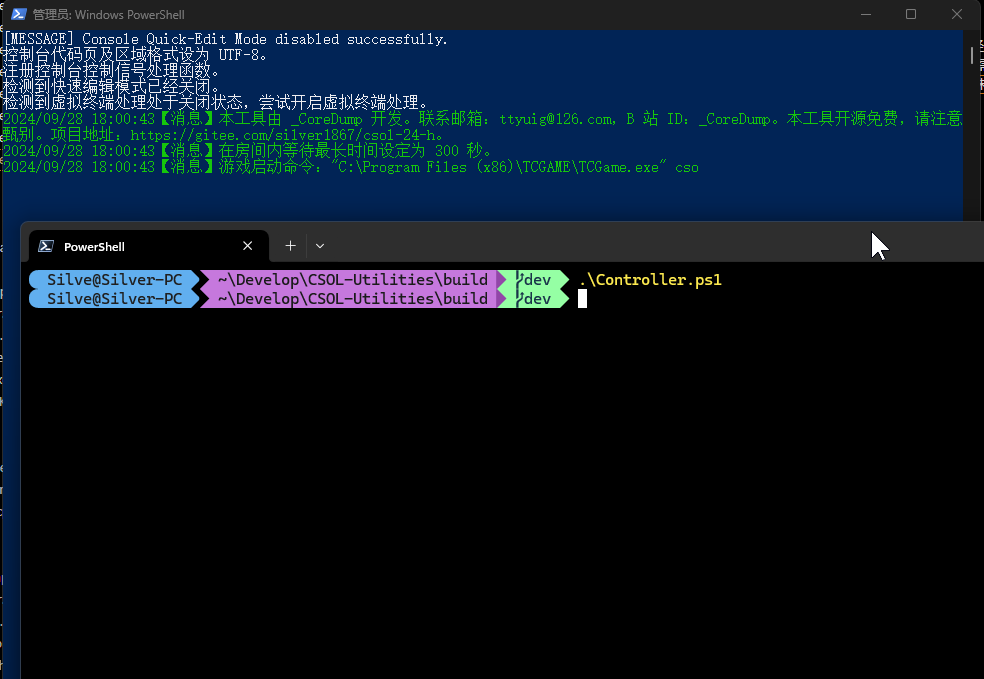
\includegraphics[width=\textwidth]{docs/assets/advanced/change_max_wait_time_in_room_1.png}
    \caption{在房间内等待的最长时间修改为 300 秒}
    \label{ch7fig-change-max-wait-time-in-room-1}
\end{figure}

\subsection{关于武器攻击}

v1.3.15 之后的版本中,\textbf{常规武器}攻击时将会调用 \lstinline{Weapon.lua} 中的 \lstinline{Weapon.attack} 方法。
该方法采用普通攻击的方式,先按下用户配置好的攻击按钮,然后在接下来的 6 秒内移动视角进行攻击,最后释放攻击按钮。

\begin{minted}[breaklines, breakautoindent]{lua}
---使用武器进行攻击攻击。
---@return nil
function Weapon:attack()
    Mouse:press(self.attack_button)
    local sensitivity_x = 1 - 0.8 * math.random() -- 水平灵敏度∈(0.2, 1]
    local sensitivity_y = 1 - 0.8 * math.random() -- 竖直灵敏度∈(0.2, 1]
    local direction = Utility:random_direction() -- 随机向左或右
    local start_time = DateTime:get_local_timestamp() -- 本次转圈开始时间
    repeat
        local t = Runtime:get_running_time() / 1000
        Mouse:move_relative(math.floor(direction * 100 * sensitivity_x), math.floor(math.sin(t) * 100 * sensitivity_y), Delay.MINI) -- 视角运动:水平方向匀速运动,竖直方向简谐运动
    until (DateTime:get_local_timestamp() - start_time > 6)
    Mouse:release(self.attack_button)
end
\end{minted}

在使用 \lstinline{Weapon.new} 方法创建武器时,您可以列表中重写 \lstinline{attack} 方法。
例如,v1.3.15 提供的 \lstinline{WeaponList.lua} 样例中,就专门为万钧神威重写了 \lstinline{attack} 方法。

\begin{minted}[breakautoindent, breaklines]{lua}
Weapon:new{
    name = "万钧神威",
    switch_delay = Delay.SHORT,
    number = Weapon.MELEE,
    purchase_sequence = {Keyboard.B, Keyboard.NINE, Keyboard.FOUR},
    -- 重写 attack 方法,按照下面定义的方式进行攻击
    attack = function ()
        Mouse:press(Mouse.RIGHT) -- 按下鼠标右键进行范围攻击
        local sensitivity_x = 1 - 0.8 * math.random() -- 水平灵敏度∈(0.2, 1]
        local sensitivity_y = 1 - 0.8 * math.random() -- 竖直灵敏度∈(0.2, 1]
        local direction = Utility:random_direction() -- 随机向左或右
        local start_time = Runtime:get_running_time() -- 本次转圈开始时间
        local first_throw = false
        local second_throw = false
        repeat
            local duration = Runtime:get_running_time() - start_time
            local t = Runtime:get_running_time() / 1000
            Mouse:move_relative(math.floor(direction * 100 * sensitivity_x), math.floor(math.sin(t) * 100 * sensitivity_y), Delay.MINI) -- 视角运动:水平方向匀速,竖直方向简谐
            if (not first_throw and 2000 < duration and duration < 4000)
            then
                Keyboard:click(Keyboard.R, Delay.SHORT)
                first_throw = true
            end
            if (not second_throw and 4000 < duration)
            then
                Keyboard:click(Keyboard.R, Delay.SHORT)
                second_throw = true
            end
        until (Runtime:get_running_time() - start_time > 4500)
        Mouse:release(Mouse.RIGHT) -- 松开鼠标右键释放旋风
    end
}
\end{minted}

对于像圣翼皓印、炽翼魔印、【幽浮】控制核心这种可以于其他武器并行攻击的\textbf{特殊武器},在创建时需要重写 \lstinline{use} 方法。
例如,\lstinline{WeaponList.lua} 样例文件中就为圣翼皓印/炽翼魔印编写了下面的 \lstinline{use} 方法。

\begin{minted}[breakautoindent, breaklines]{lua}
---特殊武器。
---@type Weapon
SpecialWeapon =
    -- 特殊武器圣翼皓印(或炽翼魔印)
    Weapon:new{
        name = "圣翼皓印/炽翼魔印",
        switch_delay = Delay.LONG_LONG,
        number = Weapon.GRENADE ,
        purchase_sequence = {Keyboard.B, Keyboard.EIGHT, Keyboard.NINE},
        discharging = false, -- 是否在释放光印
        discharge_start_moment = 0, --  光印释放的时刻。
        charge_start_moment = 0, -- 充能开始的时刻。
        DISCHARGE_TIME = 25, -- 光印释放时间。
        RECHARGE_TIME = 10, -- 充能时间。
        use = function (self)
            local current_time = DateTime:get_local_timestamp() -- 当前时间戳
            -- 当前正在充能,且充能时间超过 `RECHARGE_TIME`。
            if (not self.discharging and current_time - self.charge_start_moment > self.RECHARGE_TIME)
            then
                self.discharging = true
                self.discharge_start_moment = current_time
                self:switch()
                Mouse:click(Mouse.LEFT, 200)
            -- 当前正在释放,且释放时间超过 `DISCHARGE_TIME`。
            elseif (self.discharging and current_time - self.charge_start_moment > self.DISCHARGE_TIME)
            then
                self.discharging = false
                self.charge_start_moment = current_time
                self:switch()
                -- 按 `Keyboard.R` 召唤界徐圣。 
                Mouse:move_relative(0, 4000, Delay.NORMAL)
                Keyboard:click(Keyboard.R, 350)
                Mouse:move_relative(0, -4000, Delay.NORMAL)
            end
        end
    }\end{minted}

\subsection{关于时间}

\lstinline{DateTime.lua} 中的 \lstinline{DateTime.get_local_timestamp} 用于获取本机 UNIX 时间戳(基于世界协调时,UTC + 00:00,单位为\textbf{秒}),该方法获得的时间戳是否正确取决于 \lstinline{Setting.lua} 文件中配置的时区是否准确。
对时间精度要求不高的情况下,可以使用此函数。

\lstinline{Runtime.lua} 中的 \lstinline{Runtime.get_runnine_time} 用于获取 Lua 模块的运行时间(单位为\textbf{毫秒})。实际使用中,若您需要实现更加精确的定时控制,则可考虑使用本函数。

\subsection{关于中断机制}

罗技软件提供的 Lua 编程接口不支持多线程。
若您学过操作系统原理,则应该清楚多线程实际上需要\textbf{中断机制}来支持。
本项目的 Lua 模块通过封装罗技软件的接口,实现了一种“伪中断”机制。
鉴于发起任何键鼠操作后都需要设定一定的延迟时间(本质上是调用罗技软件提供的 \lstinline{Sleep()} 函数),本项目将 \lstinline{Sleep} 函数封装为 \lstinline{Runtime.sleep()} 方法。
调用此方法时,即认为调用方自发地中断自己的执行,随后在方法内进行中断处理。中断处理完成后,才会执行真正的睡眠,睡眠以 10 毫秒为单位进行,每过 10 毫秒又会进行一次中断处理,这也就实现了文档中提及的“即时中断”功能,
使得用户可以随意地控制 Lua 模块的启停。